\subsection{Client architecture}

The Anastasis client architecture consists of two main components. A client
API which communicates with the server and a command line application
which interacts with the user. The structure of these two components
is shown in Figure~\ref{fig:anastasis:client}.

\begin{figure}[H]
	\centering
	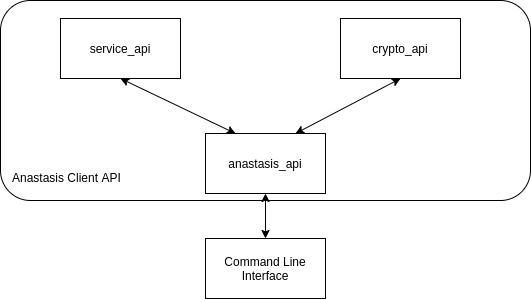
\includegraphics[scale=0.6]{images/client_api.png}
	\caption{Anastasis client architecture}
	\label{fig:anastasis:client}
\end{figure}

The Anastasis client implementation includes three distinctive APIs: a
{\em Crypto API} which provides the different cryptographic functions,
a {\em Service API} which sends the request to the server and the {\em
  Client API} which manages the main data structures and provides an
abstraction for the application.

\subsubsection{Crypto API}

The most important data structures in the crypto API are the following:

\begin{itemize}
  \item
The kdf\_id is a hash code which was generated with Argon2. The
entropy source is the user's unforgettable secret. The kdf\_id is used
to create various key's, for more details see Chapter~\ref{chap:design}.

\begin{lstlisting}
struct kdf_id
{
  Hashcode; //512-bit
}
\end{lstlisting}

\item
The account\_private\_key is used to sign the data and check the signature later. It is a 256-bit EdDSA private key. It is generated with the kdf\_id as entropy source.
\begin{lstlisting}
struct account_private_key
{
  eddsa_private_key;
}
\end{lstlisting}

\item
The account\_public\_key is used as the user identification on the different providers. It is generated from the private\_key.
\begin{lstlisting}
struct account_public_key
{
  eddsa_public_key;
}
\end{lstlisting}

\item
The truth\_key is a randomly generated AES-256 GCM key. It is used to encrypt the user specify data in the truth object.
\begin{lstlisting}
struct truth_key
{
  key; //256-bit
}
\end{lstlisting}

\item
The truth\_seed is a randomly generated nonce with a size of 32 Bytes. It is used to derive a truth\_private\_key
and is stored within an encrypted recovery document.
\begin{lstlisting}
struct truth_seed
{
  nonce; //256-bit
}
\end{lstlisting}

\item
The truth\_private\_key is used to sign the encrypted key share and the encrypted authentication data. It is a 256-bit EdDSA private key. It is generated with the truth seed as entropy source.
\begin{lstlisting}
struct truth_private_key
{
   eddsa_private_key;
}
\end{lstlisting}

The truth\_public\_key is used as the user identification on the different providers in case of uploaded truths. It is generated from the truth private key.
 \begin{lstlisting}
struct truth_public_key
{
  eddsa_public_key;
}
\end{lstlisting}


\item
Anastasis needs different symmetric keys to encrypt data for example, the recovery document. These symmetric keys are all 256-bit large hashcodes. These symmetric keys are generated through the key routine defined in Implementation Key usage.
\begin{lstlisting}
struct symmetric_key
{
  hashcode; //256-bit
}
\end{lstlisting}

\item
Each policy has a separate policy\_key. The key is used to encrypt the master\_key.
The policy\_key is also a AES-256 GCM key. It is generated through the combination of a set of key\_shares.
\begin{lstlisting}
struct policy_key
{
  hashcode; //256-bit
}
\end{lstlisting}

\item
Every truth object contains a key\_share. A key\_share is a 256-bit random generated bit sequence.
\begin{lstlisting}
struct key_share
{
  hashcode; //256-bit
}
\end{lstlisting}

\item
Before every encryption a random 256-bit large nonce is generated. This gives the encryption algorithm a random factor.
\begin{lstlisting}
struct nonce
{
  hashcode; //256-bit
}
\end{lstlisting}

\item
To use AES-256 GCM an IV must be generated. It is generated with an HKDF over a salt the kdf\_id and a symmetric key.
\begin{lstlisting}
struct iv
{
  hashcode; //128-bit
}
\end{lstlisting}

\item
The aes\_tag is generated after each encryption, it is later used to check the integrity of the data.
\begin{lstlisting}
struct aes_tag
{
  hashcode; //128-bit
}
\end{lstlisting}
\end{itemize}

The functions of the crypto API basically provide the canonical set of
cryptographic operations (hash, encrypt, decrypt, etc.)  over these
basic data structures.


\subsubsection{Client API}

The most important data structures in the client API are the following:

\begin{itemize}
  \item
The secret share data structure is used to upload a new recovery document.
\begin{lstlisting}
struct secret_share
{
  kdf_id;
  last_etag;
  policies;
  core_secret;
}
\end{lstlisting}
\begin{itemize}
\item kdf\_id: is used to compute the account public and private key. The hash is 512bit large.
\item last\_etag: this hash is sent with the recovery document. The server will check the hash if the document on the server is the same. This prevents unnecessary uploads. The hash is 512-bit large.
\item policies: is a list of all generated policies the user wants to combine into a recovery document.
\item core\_secret: is the user provided core secret. This is just a binary blob so Anastasis does not have a restriction for the user secret. This could be a for example a private key or a password the user wants to backup.
\end{itemize}

  \item
The recovery information data structure holds a recovery document. It is downloaded within the recovery process and stored inside a recovery data structure.
\begin{lstlisting}
struct recovery_information
{
  struct decryptption_policies;
  struct challenges;
  version;
  salt;
}
\end{lstlisting}
\begin{itemize}
\item decryption\_policies: holds all available policies within the downloaded recovery document.
\item challenges: holds all available authentication methods within the recovery document.
\item version: the version of the downloaded recovery document is stored here.
\item salt: this is the salt used for the generation of the policy keys. The salt is a 512-bit value.
\end{itemize}

\item
The recovery data structure is generated at the start of a secret recovery. It contains all available policies and lists which challenges are solved. Through this
struct the client can check if a policy was solved completely.
\begin{lstlisting}
struct recovery
{
  kdf_id;
  version;
  provider_url;
  salt;
  solved_challenges;
  struct recovery_information;
}
\end{lstlisting}
\begin{itemize}
\item kdf\_id: is used to compute the account public and private key. The hash is 512bit large.
\item version: hold the user desired version he wishes to download. This can be null then the client downloads the latest version.
\item provider\_url: the client will download the recovery document from this provider url.
\item salt: this is the salt of the provider specified in provider\_url.
\item solved\_challenges: this is a list of all solved challenges. This list is updated after each successful authentication. This allows the client to check if a policy is solved.
\item recovery\_information: as previously mentioned this data structure holds the downloaded recover document to process within the recovery
\end{itemize}

\item
A truth data structure is used to upload a new authentication method to a provider. It is identified by the TRUTH\_PUB which the user creates through a HKDF over the truth\_seed. The truth data structure is only used for the secret share process and not for the recovery.
\begin{lstlisting}
struct truth
{
  truth_seed;
  method;
  mime_type;
  encrypted_truth;
  encrypted_key_share;
}
\end{lstlisting}
\begin{itemize}
\item truth\_seed: the truth\_seed is the identification of the truth object.
It is used as entropy source to generate the TRUTH\_PUB, which later identificates the truth object. The truth objects are not linked to the user. A list of these truth\_seeds are stored inside the recovery document, with this the user data is more anonymous.
\item method: this defines which method the user chose to configure, for example SMS, email, secure question.
\item mime\_type: this defines in which format the truth was safed, for example jpeg, png, txt, json.
\item encrypted\_truth: the encrypted truth holds the authentication specific data. It holds for example the hashed answer and the question. It is encrypted with the specific truth\_key which is stored inside the recovery\_document.
\item encrypted\_key\_share: this is the key\_share protected by this truth. It is encrypted with a key which was derived with the kdf\_id of the user. The server will later send this key\_share to the user upon successful authentication.
\end{itemize}
\newpage
\item
The policy data structure is used to create new policies to combine them into the recovery document. The policy data structure is only used for the secret share process.
\begin{lstlisting}
struct policy
{
 truths;
 policy_key;
 salt;
}
\end{lstlisting}
\begin{itemize}
\item truths: every policy has a set of truths which need to be solved to recover the policy\_key
\item policy\_key: the policy\_key is created through the combination of the different key\_shares within each of the truth objects. It is later used to encrypt the master\_key.
\item salt: defines the salt used to create the policy\_key.
\end{itemize}

\item
The decryption\_policy data structure is used in the recovery process. It has slightly different values as the policy structure.
\begin{lstlisting}
struct decryption_policy
{
  truth_seeds;
  encrypted_master_key;
  salt;
}
\end{lstlisting}
\begin{itemize}
\item truth\_seeds: is a list of truth\_seeds which need to be solved to recreate the policy key. Each truth\_seed has a corresponding challenge.
\item encrypted\_master\_key: holds an encrypted version of the master\_key which was used to encrypt the core secret. In every policy lies the same master\_key which was encrypted by the specific policy\_key.
\item salt: defines the salt which was used to create this policy\_key.
\end{itemize}
\newpage
\item
The challenge data structure is used for the several key\_share lookups.
We named the process of authentication on the providers as challenges.
It has slightly different variables as the truth data structure.
\begin{lstlisting}
struct challenge
{
  truth_seed;
  url;
  truth_key;
  method;
  key_share;
  instructions;
}
\end{lstlisting}
\begin{itemize}
\item truth\_seed: Entropy source to generate the TRUTH\_PUB, which identifies the challenge on the server.
\item url: defines the provider URL on which the truth was stored.
\item truth\_key: this key is sent to the server within the authentication procedure. The server can decrypt the truth with this key to start the authentication.
\item method: defines the method of this challenge, for example email, SMS, secure question.
\item key\_share: After each successful authentication the key\_share which was sent by the server will be saved within this variable. It is later used to recreate a policy\_key.
\item instructions: this contains a string with the instructions for the user. This could for example be:” What is your favourite colour?” or” An SMS was sent to the number +41...... please provide the pin”.
\end{itemize}
\end{itemize}

The functions of the client API basically provide a way to
backup a core secret by providing user's identity attributes,
the secret and constructing the policies, as well as a way
to recover a core secred by providing the user's identity
attributes and then satisfying the authentication challenges.


\subsubsection{Service API}

The service API is responsible for sending the requests to the REST
API of the server. The client has implemented functions for every
endpoint.
For more details see REST API documentation in
appendix~\ref{appendix_server_api}.
